\documentclass[letterpaper, 12pt]{article}

\usepackage[utf8]{inputenc}
\usepackage[T1]{fontenc}
\usepackage{color}
\usepackage[document]{ragged2e}
\usepackage{lmodern}
\usepackage[margin=1in]{geometry}
\usepackage{amsmath,amsfonts,amssymb,amsthm}
\usepackage{mathtools}
\usepackage{graphicx}
\usepackage[shortlabels]{enumitem}
\usepackage{tikz}
\usepackage{verbatim}
\usepackage{multirow}
\usetikzlibrary{arrows,shapes}
\usepackage[%
	pdftitle={CO250 Notes},%
	hidelinks,%
]{hyperref}

%make macro for coloured text
\definecolor{red}{RGB}{210,0,0}
\definecolor{blue}{RGB}{0,0,170}
\newcommand{\red}[1]{{\color{red}{#1}}}
\newcommand{\blue}[1]{{\color{blue}{#1}}}
\newcommand{\green}[1]{{\color{green}{#1}}}
\newcommand{\yellow}[1]{{\color{yellow}{#1}}}
\newcommand{\purple}[1]{{\color{purple}{#1}}}
\newcommand{\white}[1]{{\color{white}{#1}}}

%override default second layer itemize to circle
\renewcommand{\labelitemii}{$\circ$}

\begin{document}

    
    \clearpage
    \vspace*{\fill}
    \begin{center}
        \begin{minipage}{\textwidth} 
            \title{CO250 Spring 2020}
            \author{Jacky Zhao}
            \date{\today}
            \maketitle
        \end{minipage} 
    \end{center}
    \vfill
    \thispagestyle{empty}
    \newpage
    \setcounter{page}{1}

    \section{Introduction}
    \subsection{Abstract Optimization Problem}
    An \textit{abstract optimization problem (P)} is of the following form:
    \begin{itemize}
        \item {\color{red}Given}: a set $\textbf{A} \subseteq \mathbb{R}^n$ and a function $f:\textbf{A} \rightarrow \mathbb{R}$
        \item {\color{red}Goal}: find $x \in \textbf{A}$ that minimizes/maximizes $f$
        \item {\color{red}Bad news}: Hard to solve \& may not be well defined
    \end{itemize}
    
    \bigskip
    We look at 3 special cases of (P) in this course:
    \begin{enumerate}
        \item {\color{red}Linear Programming (LP)}
        \begin{itemize}
            \item $\textbf{A}$ is simply given by \textit{linear} constrains, and $f$ is a \textit{linear} function
        \end{itemize}
        \item {\color{red}Integer Programming (IP)}
        \begin{itemize}
            \item Same as above, but now we want max/min over the \textit{integer} points in $\textbf{A}$
        \end{itemize}
        \item {\color{red}Non-linear Programming (NLP)}
        \begin{itemize}
            \item $\textbf{A}$ is given by \textit{non-linear} constrains, and $f$ is a \textit{non-linear} function
        \end{itemize}
    \end{enumerate}
    
    \subsubsection{Example: Water Tech}
    WaterTech produces 4 products, $P = \{1, 2, 3, 4\}$, from the following resources:\\
    \begin{itemize}
        \item time on two machines
        \item skilled and unskilled labour
    \end{itemize}
    The following table gives precise requirements:\\

    \bigskip
    \begin{tabular}{|c|c|c|c|c|c|}
        \hline
        Product & Machine 1 & Machine 2 & Skilled Labour & Unskilled Labour & Unit Sale Price\\
        \hline
        1 & 11 & 4 & 8 & 7 & 300\\
        \hline
        2 & 7 & 6 & 5 & 8 & 260\\
        \hline
        3 & 6 & 5 & 5 & 7 & 220\\
        \hline
        4 & 5 & 4 & 6 & 4 & 180\\
        \hline
    \end{tabular}
    \bigskip
    
    {\color{red} Restrictions:}\\
    \begin{itemize}
        \item WaterTech has 700h on machine 1 and 500h on machine 2 available
        \item it can purchase 600h of skilled labour at \$8 per hour and at most 650h of unskilled labour at \$6 per hour
    \end{itemize}
    {\color{red} Question:}\\
    How much of each product should WaterTech produce in order to maximize profit?\\
    \pagebreak
    \subsection{Ingredients of a math model:}
    \begin{itemize}
        \item {\color{red}Decision variables:} Capture unknown information
        \item {\color{red}Constraints:} Describe which assignments to variables are {\color{red}feasible}
        \item {\color{red}Objective function:} A function of the variables that we would like to maximize/minimize
    \end{itemize}

    \subsection{Variables}

    WaterTech needs to decide how many units of each product to produce, so introduce some variables:
    \begin{itemize}
        \item $x_i$ for number of labour to purchase
        \item $y_s$, $y_u$ for number of hours of skilled/unskilled labour to purchase
    \end{itemize}

    \subsection{Constrains}
    What makes an assignment to $\{x_i\} \in P, y_s, y_u$ a feasible assignment?\\
    \bigskip
    For example, a production plan described by an assignment may not use more than 700h of time on machine 1
    $$11x_1 + 7x_2 + 6x_3 + 5x_4 \leq 700$$

    Similarly, we may not use more than 500h of machine 2 time
    $$4x_1 + 6x_2 + 5x_3 + 4x_4 \leq 500$$

    Producing $x_i$ units of product $i \in P$ must require less than $y_s$ units of skilled labour
    $$8x_1 + 5x_2 + 5x_3 + 6x_4 \leq y_s$$

    Similar story for unskilled labour:
    $$7x_1 + 8x_2 + 7x_3 + 5x_4 \leq y_u$$

    Since amount of labour that can be purchased is limited, we also have
    $$y_s \leq 600$$
    $$y_u \leq 650$$

    \subsection{Objective Function}
    Revenue from sales:\\
    $$300x_1 + 260x_2 + 220x_3 + 180x_4$$

    Cost of labour:\\
    $$8y_s + 6y_u$$

    Objective Function:\\
    {\begin{center}
        maximize $300x_1 + 260x_2 + 220x_3 + 180x_4 - 8y_s - 6y_u$
    \end{center}
    \pagebreak
    
    {\large\textbf{The complete model for WaterTech problem is:}}\\
    \begin{center}
        \begin{tabular}{r l}
            max & $300x_1 + 260x_2 + 220x_3 + 180x_4 - 8y_s - 6y_u$\\
            s.t & $11x_1 + 7x_2 + 6x_3 + 5x_4 \leq 700$\\
            & $4x_1 + 6x_2 + 5x_3 + 4x_4 \leq 500$\\
            & $8x_1 + 5x_2 + 5x_3 + 6x_4 \leq y_s$\\
            & $7x_1 + 8x_2 + 7x_3 + 5x_4 \leq y_u$\\
            & $y_s \leq 600$\\
            & $y_u \leq 650$\\
            & $x_1, x_2, x_3, x_4, y_u, y_s \geq 0$\\
        \end{tabular}
    \end{center}

    Solution obtained via CPLEX is:\\
    \begin{align*}
        x &= (16 + \frac{2}{3}, 50, 0, 33 + \frac{1}{3})^T\\
        y_s &= 583 + \frac{1}{3}\\
        y_u &= 650\\
        Profit &= 15433 + \frac{1}{3}
    \end{align*}

    Notice that the solution is fractional, which may or may not be correct depending on the question\\
    \bigskip
    \subsection{Correctness of Model}
    First, define some terminologies:\\
    \begin{itemize}
        \item Word description of problem
        \begin{itemize}
            \item Similarly, a solution to the word description is an assignment to the unknowns\\
        \end{itemize}
        \item Formulation
        \begin{itemize}
            \item A solution to the formulation is an assignment to all of its variables\\
        \end{itemize}
    \end{itemize}
    
    A solution feasible if all constrains are satisfied, optimal if no other feasible solution exists\\
    \bigskip
    One way to show correctness is to define a mapping between feasible solutions to the word description, and feasible solutions to the model, and vice versa.\\
    \pagebreak

    \section{Linear Program Model (LP)}

    \subsection{Linear Functions}
    Affine Functions
    \begin{itemize}
        \item A function $f : \mathbb{R}^n \rightarrow \mathbb{R}$ is affine if $f(x) = \alpha^Tx + \beta$ for $\alpha \in \mathbb{R}^n, \beta \in \mathbb{R}$
    \end{itemize}
    Linear Functions
    \begin{itemize}
        \item An affine function with $\beta = 0$
    \end{itemize}

    \subsection{Linear Program}
    Linear Program
    \begin{itemize}
        \item the optimization problem $$max/min\{f(x):f_i(x) \leq b_i, \forall1 \leq i \leq m, x \in \mathbb{R}^n\}$$ is a linear program if $f$ is affine and $g_1,...,g_m$ is finite number of linear functions\\
    \end{itemize}
    
    \bigskip
    Some notes:
    \begin{itemize}
        \item dividing by variables is not allowed in LP
        \item can NOT have strict inequalities
        \item must have FINITE number of constraints
    \end{itemize}
    
    Example:\\
    \bigskip
    \begin{tabular}{rl}
        max & $\frac{-1}{x_1} - x_3$\\
        s.t. & $2x_1 + x_3 < 3$\\
        &$x_1 + \alpha x_2 = 2\hspace{1cm}\forall\alpha\in\mathbb{R}$\\
    \end{tabular}
    \bigskip

    Going back to the WaterTech problem, the model we created was in fact a linear program!\\

    \subsection{LP Models: Multiperiod Models}
    A multiperiod model is a problem where:\\
    \begin{itemize}
        \item time is split into periods
        \item we have to make a decision in each period
        \item all decisions influences the final outcome
    \end{itemize}
    Example:\\
    KW Oil is a local supplier of heating oil, it needs to decide how much oil to purchase in order to satisfy demand of its customers.\\
    \bigskip
    \begin{tabular}{|c|c|c|c|c|}
        \hline
        Month & 1 & 2 & 3 & 4\\
        \hline
        Demand($l$) & 5000 & 8000 & 9000 & 6000\\
        \hline
        Price(\$/$l$) & 0.75 & 0.72 & 0.92 & 0.90\\
        \hline
    \end{tabular}
    \bigskip

    Question: When should we purchase how much oil when the goal is to min overall total cost?\\
    Additional Complication: The company has a storage tank that\\
    \begin{itemize}
        \item has a capacity of 4000 litres of oil
        \item currently (beginning of month 1) contains 2000 litres of oil
    \end{itemize}
    Assumption: Oil is delivered at the beginning of the month, and consumption occurs int he middle of the month

    \bigskip
    {\large\textbf{Variables}}
    \begin{itemize}
        \item Need to decide how many litres of oil to purchase in each month $i$
        \begin{itemize}
            \item make variable $p_i$ for $i \in [4]$
        \end{itemize}
        \item How much oil is stored in the tank at the beginning of month $i$?
        \begin{itemize}
            \item make variable $t_i$ for $i \in [4]$
        \end{itemize}
    \end{itemize}

    {\large\textbf{Objective Function}}\\
    Minimize cost of oil purchased
    $$min\hspace{1cm} 0.75p_1 + 0.72p_2 + 0.92p_3 + 0.90p_4$$

    {\large\textbf{Constrains}}\\
    We need 
    \begin{center}
        $p_i + t_i \geq$ (demand in month $i$)\\
    \end{center}
    Balancing equation we get
    \begin{center}
        $p_i + t_i = $ (demand in month $i$) $ + t_{i+1}$\\
    \end{center}

    So we have the following four constrains
    \begin{align*}
        p_1 + 2000 & = 5000 + t_2\\
        p_2 + t2 & =  5000 + t_3\\
        p_3 + t3 & =  5000 + t_4\\
        p_4 + t4 & \geq  6000
    \end{align*}

    {\large\textbf{Complete LP for KW Oil}}\\
    \bigskip
    \begin{tabular}{rl}
        min & $0.75p_1 + 0.72p_2 + 0.92p_3 + 0.90p_4$\\
        s.t. & {$\begin{aligned}[t]
            p_1 + 2000 & = 5000 + t_2\\
            p_2 + t2 & =  5000 + t_3\\
            p_3 + t3 & =  5000 + t_4\\
            p_4 + t4 & \geq  6000\\
            t_1 &= 2000\\
            t_i &\leq 4000 \hspace{1cm} (i=2, 3, 4)\\
            t_1, p_i &\geq 0 \hspace{1cm} (i=1, 2, 3, 4) \end{aligned}$}
    \end{tabular}
    \bigskip
    
    Solving the LP gives the solution:\\
    $p = (3000,12000,5000,6000)^T$\\
    $t = (2000, 0, 4000, 0)^T$

    \pagebreak
    \section{Integer Program (IP)}
    Recall the WaterTech problem\\
    \begin{center}
        \begin{tabular}{r l}
            max & $300x_1 + 260x_2 + 220x_3 + 180x_4 - 8y_s - 6y_u$\\
            s.t & $11x_1 + 7x_2 + 6x_3 + 5x_4 \leq 700$\\
            & $4x_1 + 6x_2 + 5x_3 + 4x_4 \leq 500$\\
            & $8x_1 + 5x_2 + 5x_3 + 6x_4 \leq y_s$\\
            & $7x_1 + 8x_2 + 7x_3 + 5x_4 \leq y_u$\\
            & $y_s \leq 600$\\
            & $y_u \leq 650$\\
            & $x_1, x_2, x_3, x_4, y_u, y_s \geq 0$\\
        \end{tabular}
    \end{center}

    \begin{align*}
        x &= (16 + \frac{2}{3}, 50, 0, 33 + \frac{1}{3})^T\\
        y_s &= 583 + \frac{1}{3}\\
        y_u &= 650\\
        Profit &= 15433 + \frac{1}{3}
    \end{align*}

    Fractional solutions are often not desirable! Can we force the solution to be integer?\\
    \bigskip
    {\large\textbf{Integer Program}}\\
    \begin{itemize}
        \item an integer program is a linear program with added integrality constraints for some/all the variables
        \item we call an IP mixed if there are integer and fractional variables, and pure otherwise
        \item the difference between LPs and IPs is subtle, but LPs are easy to solve, IPs are not!
    \end{itemize}
    Integer program is provably difficult to solve!\\
    \begin{itemize}
        \item An algorithm is efficient if its running can be bounded by a polynomial of the input size of the instance\\
        \item LPs can be solved efficiently
        \item IPs are very unlikely to have efficient algorithms!
    \end{itemize}

    \pagebreak
    \subsection{IP Models: Knapsack}
    Example:\\
    KitchTech Shipping is a company wishes to ship crates from Toronto to Kitchener.
    Each crate type has a weight and value, and the total weight of crates shipped must not exceed 10,000 lbs.\\
    Goal: Maximize the total value of shipped goods.\\
    \bigskip
    \begin{center}
        \begin{tabular}{|c|c|c|c|c|c|c|}
            \hline
            Type & 1 & 2 & 3 & 4 & 5 & 6\\
            \hline
            weight (lbs) & 30 & 20 & 30 & 90 & 30 & 70\\
            \hline
            value (\$) & 60 & 70 & 40 & 70 & 20 & 90\\
            \hline
        \end{tabular}
    \end{center}

    \bigskip
    \textbf{Variables:}\\
    One variable $x_i$ for the number of crates of type $i$ to pack.\\
    \bigskip
    \textbf{Constraints:}\\
    The total weight of crates picked must not exceed 10000 lbs.\\
    $$30x_1 + 20x_2 + 30x_3 + 90x_4 + 30x_5 + 70x_6 \leq 10000$$
    \textbf{Objective function:}\\
    Maximize the total value\\
    $$max \hspace{1cm} 60x_1 + 70x_2 + 40x_3 + 70x_4 + 20x_5 + 90x_6$$

    \textbf{Complete IP model for KitchTech Shipping:}\\
    \begin{center}
        \begin{tabular}{rl}
            max & $60x_1 + 70x_2 + 40x_3 + 70x_4 + 20x_5 + 90x_6$\\
            s.t. & $30x_1 + 20x_2 + 30x_3 + 90x_4 + 30x_5 + 70x_6 \leq 10000$\\
            & $x_i \geq 0 \hspace{1cm} (i\in[6])$\\
            & $x_i$ integer $(i \in [6])$\\
        \end{tabular} 
    \end{center}
    
    Let's make this shit more complicated with more rules...\\
    Suppose that:
    \begin{enumerate}
        \item we must not send more than 10 crates of the same type
        \item we can only send crates of type 3, if we send at least 1 crate of type 4
    \end{enumerate}}
    Note that we can send at most 10 crates of type 3 by the previous constraints!\\
    By adding the following constraint, the added requirements is fulfilled:
    $$ x_3 \leq 10x_4$$

    \pagebreak
    \textbf{proving correctness of the added constraint:}
    \begin{itemize}
        \item $x_4 \geq 1 \rightarrow$  new constraint is redundant
        \item $x_4 = 0 \rightarrow$  new constraint becomes $x_3 \leq 0$
    \end{itemize}

    Suppose we add another rule where we must:\\
    \begin{enumerate}
        \item take a total of at least 4 crates of type 1 or 2, or
        \item take at least 4 crates of type 5 or 6
    \end{enumerate}

    \textbf{strategy:}\\
    Create a new variable y such that:
    \begin{itemize}
        \item $y = 1 \rightarrow x_1 + x_2 \geq 4$
        \item $y = 0 \rightarrow x_5 + x_6 \geq 4$
        \item and force $y$ to take on value 0 or 1
    \end{itemize}

    So we add the following constraints:\\
    \begin{itemize}
        \item $x_1 + x_2 \geq 4y$
        \item $x_5 + x_6 \geq 4(1 - y)$
        \item $0 \leq y \leq 1$
        \item y integer
    \end{itemize}

    The variable $y$ we added is called a binary variable. These are very useful for modelling logical constraints of the form:\\
    \begin{itemize}
        \item Condition (A or B) and C $\rightarrow$ D
    \end{itemize}

    So the finalized model would be:\\
    \begin{center}
        \begin{tabular}{rl}
            max & $60x_1 + 70x_2 + 40x_3 + 70x_4 + 20x_5 + 90x_6$\\
            s.t. & $30x_1 + 20x_2 + 30x_3 + 90x_4 + 30x_5 + 70x_6 \leq 10000$\\
            & $ x_3 \leq 10x_4$\\
            & $x_1 + x_2 \geq 4y$\\
            & $x_5 + x_6 \geq 4(1 - y)$\\
            & $x_i \geq 0 \hspace{1cm} (i\in[6])$\\
            & $0 \leq y \leq 1$\\
            & y integer\\
            & $x_i$ integer $(i \in [6])$\\
        \end{tabular} 
    \end{center}
    \pagebreak
    \subsection{IP Models: Scheduling}
    Example:\\
    The neighborhood coffee shop is open on workdays. The daily demand for workers is given in the table.
    Each worker works for 4 consecutive days and has one day off.\\
    Goal: Hire the smallest number of workers so that the demand can be met\\
    \bigskip
    \begin{tabular}{|c|c|c|c|c|}
        \hline
        Mon & Tues & Wed & Thurs & Fri\\
        \hline
        3 & 5 & 9 & 2 & 7\\
        \hline
    \end{tabular}
    
    \bigskip
    \textbf{Variables:}\\
    Introduce variable $x_d$ for every $d \in \{M,T,W,Th,F\}$ counting the number of people to hire with starting day $d$\\
    \bigskip
    \textbf{Objective function:}\\
    Minimize the total number of people hired:\\
    $$min \hspace{1cm} x_M + x_T + x_W + x_{Th} + x_F$$
    \textbf{Constraints:}\\
    We need to ensure that enough people work on each of the days.\\
    \textbf{Question:} Given a solution, how many people work on Monday?\\
    \textbf{Answer:} All but those that start on Tuesday, i.e.
    $$x_M + x_W + x_{Th} + x_F$$
    And it must be greater than or equal to the number of workers required\\
    So the complete LP is:\\
    \bigskip
    \begin{center}
        \begin{tabular}{rl}
            min & $x_M + x_T + x_W + x_{Th} + x_F$\\
            s.t. & $x_M + x_W + x_{Th} + x_F \geq 3$\\
            & $x_M + x_T + x_{Th} + x_F \geq 5$\\
            & $x_M + x_T + x_W + x_F \geq 9$\\
            & $x_M + x_T + x_W + x_{Th} \geq 2$\\
            &  $x_T + x_W + x_{Th} + x_F \geq 7$\\
            & $x \geq 0, x$ integer\\
        \end{tabular}
    \end{center}
    
    \pagebreak
    \section{Optimization on graphs}
    \subsection{Graph Theory 101:}
    A graph G consist of:
    \begin{itemize}
        \item vertices $u,w,...\in V$ (circles)
        \item edges $uw,wz,...\in E$ (lines connecting circles)
    \end{itemize}
    Two vertices $u$ and $v$ are adjacent if $uv \in E$.\\
    Vertices $u$ and $v$ are the endpoints of edge $uv \in E$\\
    An edge $e \in E$ is incident to $u \in V$ if $u$ is an endpoint of $e$.\\
    \bigskip
    An $s,t-path$ in $G = (V,E)$ is a sequence
    $$v_1v_2,v_2v_3,v_3v_4,...,v_{k-2}v_{k-1},v_{k-1}v_k$$
    Where\\
    \begin{itemize}
        \item $v_i \in V$ and $v_iv_{i+1} \in E$ for all $i$, and
        \item $v_1 = s, v_k = t$ and $\underbrace{v_i \neq v_j \text{ for all } i \neq j}_{\text{Without this, it is called an s,t-walk}}$
    \end{itemize}
    The length of a path $P = v_1v_2,v_2v_3,v_3v_4,...,v_{k-1}v_k$ is the sum of the lengths of the edges on P
    $$c(P) = \sum(c_e:e \in P)$$
    
    \subsection{IP Models: Matchings}
    Example:\\
    WaterTech has a collection of important jobs that it needs to handle urgently.\\
    It also has 4 employees that need to handle these jobs.\\
    Employees have different skill-sets and may take different amount of times to execute a job, note that
    some workers are not able to handle certain jobs!\\
    \bigskip
    \textbf{Goal:} Assign each worker to exactly one task so that the total execution time is smallest!\\
    We will rephrase this in the language of graphs.\\
    \bigskip
    \begin{center}
        \begin{tabular}{|c|c|c|c|c|}
            \hline
            \multirow{2}{*}{Employees} & \multicolumn{4}{|c|}{Jobs}\\
            \cline{2-5}
            & 1' & 2' & 3' & 4'\\
            \hline
            1 & - & 5 & - & 7\\
            2 & 8 & - & - & 4\\
            3 & - & 1 & - & -\\
            4 & 8 & - & 3 & -\\
            \hline
        \end{tabular}
    \end{center}
    \bigskip

    Create a graph with one vertex for each employee and job.\\
    Add an edge $ij$ with cost $c_{ij}$ for $i \in E$ and $j \in J$ if employee $i$ can handle job $j$ in time $c_{ij}$\\

    \begin{center}
        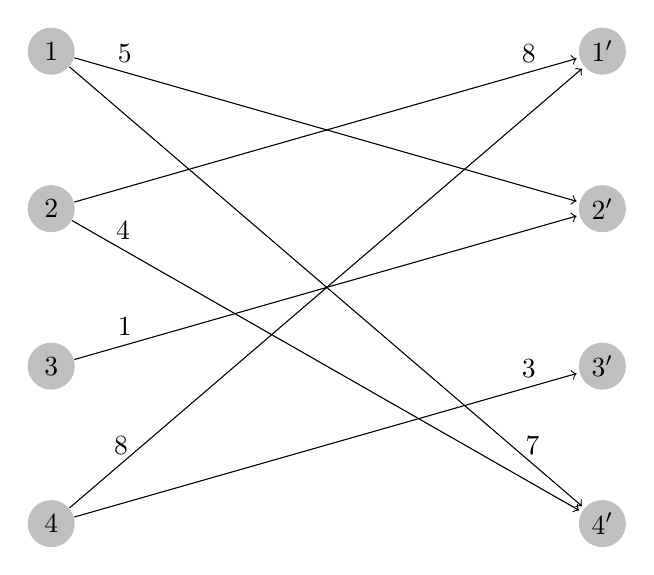
\begin{tikzpicture}[shorten >=1pt,->]
            \tikzstyle{vertex}=[circle,fill=black!25,minimum size=17pt,inner sep=0pt]
          
            \foreach \name/\x in {1/4, 2/3, 3/2, 4/1}
              \node[vertex] (G-\name) at (0, 2*\x) {$\name$};
    
            \foreach \name/\x in {1'/4, 2'/3, 3'/2, 4'/1}
              \node[vertex] (G-\name) at (7, 2*\x) {$\name$};
          
            \foreach \from/\to/\value in {1/2'/5, 2/4'/4, 4/1'/8,3/2'/1}
              \draw (G-\from) -- (G-\to) node[pos=0.1, above] {\value};
    
            \foreach \from/\to/\value in {1/4'/7, 2/1'/8,  4/3'/3}
              \draw (G-\from) -- (G-\to) node[pos=0.9, above] {\value};
        \end{tikzpicture}
    \end{center}
    
    \textbf{Matching}
    \begin{itemize}
        \item A collection $M \subseteq E$ is matching if no two edges $ij, i'j' \in M (ij \neq i'j')$ share an endpoint.
        \item i.e. $\{ij\} \cap \{i'j'\} = 0$
    \end{itemize}
    For example:
    \begin{itemize}
        \item $M = \{14', 21', 32', 43'\}$ is a matching
        \item $M = \{14', 32', 41', 43'\}$ is NOT a matching
    \end{itemize}

    The cost of a matching $M$ is the sum of costs of its edges:
    $$c(M) = \sum (c_e : e \in M)$$

    A matching $M$ is \red{perfect} if every vertex $v$ in the graph is incident to an edge in $M$\\
    Note: a perfect matching correspond to feasible assignments of workers to jobs!\\
    \bigskip
    \textbf{More notations:}\\
    Use $\delta(v)$ to denote the set of edges incident to $v$, i.e.:
    $$ \delta(v) = \{e \in E : e = vu \text{ for some } u \in V\}$$
    \red{This definition is improved later!}\\
    For example:\\
    \begin{itemize}
        \item $\delta(2) = \{21', 24'\}$
        \item $\delta(3') = \{43'\}$
    \end{itemize}
    \pagebreak
    So another definition of a \red{perfect matching} is:
    \begin{itemize}
        \item Given $G = (V,E), M \subseteq E$ is a perfect matching \red{iff $M \cap \delta(v)$ contains a single edge} for all $v \in V$
    \end{itemize}

    So the IP will have a binary variable $x_e$ for every edge $e \in E$, the idea is:\\
    \begin{itemize}
        \item $x_e = 1 \longleftrightarrow e \in M$
    \end{itemize}

    So the constraints for perfect matching is:\\
    For all $v \in V$, we need
    $$\sum (x_e : e \in \delta(v)) = 1$$
    The objective function would be:\\
    $$\sum(c_ex_e : e \in E)$$

    \textbf{Complete IP for any perfect matching problem:}\\
    \begin{center}
        \begin{tabular}{rl}
            min & $\sum (c_ex_e : e\in E)$\\
            s.t & $\sum (x_e : e \in \delta(v)) = 1 (v \in V)$\\
            & $x \geq 0$, x is integer
        \end{tabular}
    \end{center}

    \textbf{For the example question, we have:}\\
    \begin{center}
        \begin{tabular}{rl}
            min & $(5,1,3,4)x)$\\
            s.t & \begin{tabular}{cccccccc}
                & \multicolumn{6}{c}{\multirow{5}{*}{\begin{tabular} {@{}cccccc@{}}
                    & 12 & 13 & 14 & 23 &\\
                    \multirow{4}{*}{$\Big($}
                    & 1 & 1 & 1 & 0 &
                    \multirow{4}{*}{$\Big)$}\\
                    & 1 & 0 & 0 & 1 &\\
                    & 0 & 1 & 0 & 1 &\\
                    & 0 & 0 & 1 & 0 &\\
                \end{tabular}}}\\
                1 &&&&&&&\multirow{4}{*}{$x = \mathbf{1}$}\\
                2\\
                3\\
                4\\
            \end{tabular}\\
            & $x \geq 0$, x is integer
        \end{tabular}
    \end{center}

    \subsection{Shortest Path Problem}

    Input:\\
    \begin{itemize}
        \item Graph $G = (V,E)$
        \item Non-negative \red{edge lengts} $c_e$ for all $e \in E$
        \item Vertices $s,t \in V$
    \end{itemize}

    Goal: Compute an $s,t$-path of the smallest total length\\

    \bigskip
    The shortest path problem is:
    \begin{itemize}
        \item Given: Graph $G = (V,E)$, lengths $c_e \geq 0$ for all $e \in E$, and $s,t \in V$, compute an $s,t$-path of smallest total length
    \end{itemize}
    
    Useful Observation:\\
    \begin{itemize}
        \item Let $C \in E$ be a set of edges whose removal \red{disconnects} $s$ and $t$
    \end{itemize}
    
    For example:\\
    
    \begin{center}
        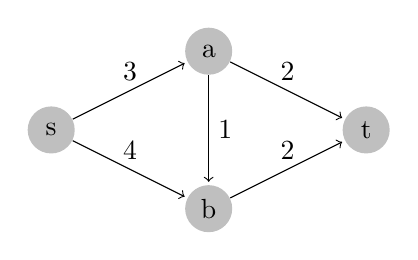
\begin{tikzpicture}[shorten >=1pt,->]
            \tikzstyle{vertex}=[circle,fill=black!25,minimum size=17pt,inner sep=0pt]
          
            \node[vertex] (G-s) at (0, 1) {s};
            \node[vertex] (G-a) at (2, 2) {a};
            \node[vertex] (G-b) at (2, 0) {b};
            \node[vertex] (G-t) at (4, 1) {t};
          
            \draw (G-s) -- (G-a) node[pos=0.5, above] {3};
            \draw (G-s) -- (G-b) node[pos=0.5, above] {4};
            \draw (G-a) -- (G-t) node[pos=0.5, above] {2};
            \draw (G-b) -- (G-t) node[pos=0.5, above] {2};
            \draw (G-a) -- (G-b) node[pos=0.5, right] {1};
        \end{tikzpicture}
    \end{center}

    Let $C = \{sb, ab, at\}$, notice that removing all edges in $C$ eliminates all paths from $s$ to $t$\\
    Therefore, \red{every $s,t$-path must have at least one edge in $C$}\\
    \bigskip
    A more precise definition of notation $\delta$:\\
    For $S \in V$, we let $\delta(S)$ be the set of edges with \red{exactly one endpoint in $S$}\\
    $$\delta(S) = \{uv \in E : u \in S, v \notin S\}$$

    Examples:\\
    \begin{enumerate}
        \item $S =\{s\} \rightarrow \{sa, ab\}$
        \item $S =\{s, a\} \rightarrow \{ab, at, sb\}$
        \item $S =\{a, b\} \rightarrow \{sa, sb, at, bt\}$
    \end{enumerate}

    Definition of \red{$s,t$-cut}:\\
    \begin{itemize}
        \item $\delta(S)$ is an $s,t$-cut if $s \in S$ and $t \notin S$
    \end{itemize}
    
    Using the 3 $\delta(S)$ examples above, 1 and 2 are $s,t$-cuts, 3 is not\\

    \bigskip
    \textbf{Remark:}
    \begin{enumerate}
        \item if $P$ is an $s,t$-path and $\delta(S)$ is an $s,t$-cut, then P \red{must have an edge} from $\delta(S)$
        \item if $S \subseteq E$ contains \red{at least one} edge from \red{every $s,t$-cut}, then $S$ contains an $s,t$-path
    \end{enumerate}
    \pagebreak
    Prove \#2 by contradiction:\\
    \begin{itemize}
        \item suppose $S$ has an edge from every $s,t$-cut, but $S$ has no $s,t$-path
        \item Let $R$ be the set of vertices \red{reachable} from $s$ in $S$: $R = \{u \in V : S \text{ has an }s,u \text{ path}\}$
        \item $\delta(R)$ is an $s,t$-cut since $s \in R$ and $t \notin R$
        \item Note: there cannot be an edge $uv \in S$ with $u \in R$ and $v \notin R$. Otherwise $v$ should have been in $R$!
        \item So $\delta(R) \cap S = \emptyset$
        \item Contradiction!
    \end{itemize}

    \textbf{Generic IP for Shortest Path problem:}\\
    \red{\textbf{Variables:}}\\ 
    We have one binary variable $x_e$ for each edge $e \in E$. We want:\\
    $$x_e = \left\{ \begin{array}{ll}
        1 & : e \in P\\
        0 & : \text{otherwise}\\
        \end{array}
    \right.$$
    \red{\textbf{Constraints:}}\\
    We have one constraint for each $s,t$-cut $\delta(U)$, forcing $P$ to have an edge from $\delta(S)$\\
    \begin{equation}
        \sum x_e : e \in \delta(U)) \geq 1 \hspace{1cm}\text{for all $s,t$-cuts $\delta(U)$}
    \end{equation}

    \red{\textbf{Objective Function:}}\\
    $$\sum(c_ex_e : e \in E)$$

    \red{\textbf{Complete Model:}}\\
    \begin{center}
        \begin{tabular}{rl}
            min & $\sum(c_ex_e : e \in E)$\\
            s.t. & $\sum(x_e : e \in \delta(U)) \geq 1 (U \subseteq V, s \in U, t \notin U)$\\
            & $x_e \geq 0$, $x_e$ integer\\
        \end{tabular}
    \end{center}

    Suppose $c_e > 0$ for all $e \in E$, then in an optimal solution, $x_e \leq 1$ for all $e \in E$\\
    \begin{itemize}
        \item Suppose $x_e \geq 1$
        \item Then let $x_e = 1$. This is cheaper and maintains feasibility!
    \end{itemize}

    For binary solution $x$, define\\
    $$S_x = \{e \in E : x_e = 1\}$$
    Note: If $x$ is a feasible for an IP, then $S_x$ has at least one edge from every $s,t$-cut and $S_x$ has a $s,t$-path, \red{but} $S_x$ may contain more than just an $s,t$-path!
    \pagebreak
    Consider this diagram again:
    \begin{center}
        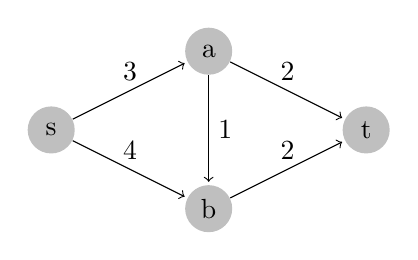
\begin{tikzpicture}[shorten >=1pt,->]
            \tikzstyle{vertex}=[circle,fill=black!25,minimum size=17pt,inner sep=0pt]
          
            \node[vertex] (G-s) at (0, 1) {s};
            \node[vertex] (G-a) at (2, 2) {a};
            \node[vertex] (G-b) at (2, 0) {b};
            \node[vertex] (G-t) at (4, 1) {t};
          
            \draw (G-s) -- (G-a) node[pos=0.5, above] {3};
            \draw (G-s) -- (G-b) node[pos=0.5, above] {4};
            \draw (G-a) -- (G-t) node[pos=0.5, above] {2};
            \draw (G-b) -- (G-t) node[pos=0.5, above] {2};
            \draw (G-a) -- (G-b) node[pos=0.5, right] {1};
        \end{tikzpicture}
    \end{center}
    Let $x_e = 1$ for $e \in \{sa, ab, at\}$, and $x_e = 0$ otherwise.\\
    So $S_x = \{sa, ab, at\}$\\
    $x$ cannot be optimal for the IP because we can reduce $S_x$ and get a better solution!\\
    i.e. let $x_ab = 0$ and the solution is more efficient\\
    \bigskip
    So if $x$ is an optimal solution for the IP \red{and $c_e \geq 0$ for all $e \in E$} then $S_x$ contains the edges of a shortest $s,t$-path

    \pagebreak
    \section{Nonlinear Programs (NLP)}
    A nonlinear program (NLP) is of the form:\\
    \begin{center}
            \begin{tabular}{rl}
                min & $f(x)$\\
                s.t. & $g_1(x) \leq 0$\\
                & $g_2(x) \leq 0$\\
                & $\dots$\\
                & $g_m(x) \leq 0$\\
            \end{tabular}
    \end{center}

    Where:\\
    \begin{itemize}
        \item $x \in \mathbb{R}$
        \item $f : \mathbb{R}^n \rightarrow \mathbb{R}$
        \item $g_i : \mathbb{R}^n \rightarrow \mathbb{R}$
    \end{itemize}
    
    \red{Note:} Linear programs (LPs) are NLPs!\\

    \subsection{NLP Models: Finding Close Points in an LP}
    \red{\textbf{Problem:}}\\
    We are given an LP (P), and an infeasible point $\bar{x}$\\
    \red{\textbf{Goal:}}\\
    Find a point $x \in P$ that is as close as possible to $\bar{x}$\\
    \bigskip
    i.e. find a point $x \in P$ that minimizes the \red{Euclidean distance} to $\bar{x}$\\
    $$||x - \bar{x}||_2 = \sqrt{\sum^n_{i=1}(x_i - \bar{x}_i)^2}$$
    Remark: $||p||_2$ is called the $L^2$-norm of p

    \bigskip
    \red{\textbf{Generic model:}}\\
    \begin{center}
        \begin{tabular}{c|c}
            \begin{tabular}[t]{rl}
                \multicolumn{2}{l}{Given LP:}\\
                min & $c^Tx$\\
                s.t. & $x \in P$
            \end{tabular} & \begin{tabular}[t]{rl}
                \multicolumn{2}{l}{Solve:}\\
                min & $||x - \bar{x}||_2$\\
                s.t. & $x \in P$ where $P = \{x: Ax \leq b\}$\\
            \end{tabular}
        \end{tabular}
    \end{center}

    \subsection{NLP Models: Binary IPs}
    Suppose we are given a binary IP (i.e. an IP with all variables are binary)\\
    Recall that Binary IPs are generally hard to solve!\\
    We need to rewrite binary IPs as NLPs\\
    \bigbreak
    \red{\textbf{Generic model:}}\\
    \begin{center}
        \begin{tabular}{c|c}
            \begin{tabular}[t]{rl}
                \multicolumn{2}{l}{Given IP:}\\
                max & $c^Tx$\\
                s.t. & $Ax \leq b$\\
                & $x \geq 0$\\
                & $x_j \in \{0,1\} \hspace{1cm} (j \in \{1,/dots,n\})$\\
            \end{tabular} & \begin{tabular}[t]{rl}
                \multicolumn{2}{l}{Rewrite:}\\
                max & $c^Tx$\\
                s.t. & $Ax \leq b$\\
                & $x \geq 0$\\
                & $x_j(1-x_j) = 0 \hspace{1cm} (j \in [n]) \hspace{1cm} (*)$\\
            \end{tabular}
        \end{tabular}
    \end{center}
    \bigskip
    Correctness:\\
    For $j \in [n]$, $(*)$ holds iff $x_j = 0$ or $x_j = 1$\\
    \bigskip
    Question:\\
    Can you change the NLP to express teh fact that $x_j$ is \red{any non-negative integer} instead of binary?\\
    \begin{center}
        \begin{tabular}{rl}
            max & $c^Tx$\\
            s.t. & $Ax \leq b$\\
            & $x \geq 0$\\
            & $sin(\pi x_j) = 0 \hspace{1cm} (j \in [n]) \hspace{1cm} (**)$\\
        \end{tabular}
    \end{center}
    \bigskip
    Correctness:\\
    Note that $sin(\pi x_j) = 0$ only if $x_j$ is an integer. 
    Combining with non negative constraint it limits $x_j$ to be any non-negative integer.\\

    \subsection{Fermat's last Theorem}
    Conjecture:\\
    There are \red{no integers $x,y,z \geq 1$ and $n \geq 3$} such that\\
    $$x^n + y^n = z^n$$
    The proof is 150 pages long!\\
    \bigskip
    \textbf{NLP for Fermat's Last Theorem}\\
    \begin{center}
        \begin{tabular}{rl}
            min & $({x_1}^{x_4} + {x_2}^{x_4} - {x_3}^{x_4}) ^2 + (sin \; \pi x_1)^2 + (sin \; \pi x_2)^2 + (sin \; \pi x_3)^2 + (sin \; \pi x_4)^2$\\
            s.t. & $x_i \geq 1 \hspace{1cm} (i = 1\dots3)$\\
            & $x_4 \geq 3$\\
        \end{tabular}
    \end{center}
    \pagebreak
    \begin{itemize}
        \item This NLP is trivially feasible, and the value of any feasible solution is non-negative as its objective is the \red{sum of squares}, which means the min possible value is 0
        \item In fact, the value of a solution $(x_1, x_2, x_3, x_4)$ is 0 iff
        \begin{itemize}
            \item ${x_1}^{x_4} + {x_2}^{x_4} = {x_3}^{x_4}$, and
            \item $(sin \; \pi x_i)^2 = 0$, for all $(i = 1 \dots 3)$
        \end{itemize}
    \end{itemize}

    \red{\textbf{Notes:}}\\
    \begin{itemize}
        \item Fermat's Last Theorem is true iff the NLP has optimal value \red{greater than} 0
        \item It is well known that there is an infinite sequence of feasible solutions whose objective value converges to 0!
        \item To prove Fermat's Last Theorem we must show that the value 0 \red{can not be attained!}
    \end{itemize}

    \pagebreak
    
    \section{Linear Programs: Possible Outcomes}
    What does solving an optimization problem mean?\\
    \boxed{\text{LP/IP/NLP}} $\rightarrow$ \boxed{\text{algorithm (software)}} $\rightarrow$ \boxed{\text{solution}}\\
    \bigskip

    For example:\\
    \begin{tabular}{rl}
        max & $2x_1 - 3x_2$\\
        s.t. & $x_1 + x_2 \leq 1$\\
        & $x_1, x_2 \geq 0$\\
    \end{tabular}\\
    \bigskip
    Trivially, the solution for this problem is:\\
    \begin{tabular}{l}
        $x_1 = 1$\\
        $x_2 = 0$\\
    \end{tabular}
    But sometimes, the answer is not so straightforward!\\

    \subsection{3 types of outcomes}

    \red{\textbf{Feasibility}}\\
    \begin{itemize}
        \item a assignment of values to each of the variables is a \red{feasible solution} if all the constraints are satisfied
        \item an optimization problem is \red{feasible} if it has at least one feasible solution
        \item It is \red{infeasible} otherwise
    \end{itemize}
    Note: a feasible optimization problem can have infeasible solutions!\\
    \bigskip
    \red{\textbf{Optimal}}\\
    \begin{itemize}
        \item For a maximization problem, an \red{optimal solution} is a feasible solution that max the objective function.
        \item For a minimization problem, an \red{optimal solution} is a feasible solution that min the objective function.
    \end{itemize}

    Notes:\\
    \begin{itemize}
        \item an optimization problem can have several optimal solutions!
        \item an infeasible problem can NOT have optimal solutions
        \item not every feasible problem have an optimal solution
    \end{itemize}

    Examples:\\
    \begin{tabular}{|rl|l}
        \cline{1-2}
        max & $x_1$ & \multirow{3}{*}{Infeasible problem, so no optimal solution}\\
        s.t & $x1 \geq 2$\\
        & $x_1 \leq 1$\\
        \cline{1-2}
    \end{tabular}
    \bigskip\\
    \begin{tabular}{|rl|l}
        \cline{1-2}
        max & $x_1$ & Feasible $x_1 = 1$, but still no optimal solution\\
        s.t & $x1 \geq 1$ & Also called unbounded problem\\
        \cline{1-2}
    \end{tabular}
    \pagebreak

    \red{\textbf{Unboundedness:}}\\
    \begin{itemize}
        \item A maximization problem is \red{unbounded} if for every value $M$, there exists
         a feasible solution with objective value greater than $M$
        \item A minimization problem is \red{unbounded} if for every value $M$, there exists 
         a feasible solution with objective value smaller than $M$
    \end{itemize}

    Note:\\
    There exist problems that are NOT infeasible, NO optimal solution, and NOT unbounded\\
    \bigskip
    For example:\\
    \begin{tabular}{rl}
        max & $x$\\
        s.t. & $x < 1$\\
    \end{tabular}
    \begin{itemize}
        \item It is feasible as $x = 0$ is a feasible solution
        \item It is not unbounded since $1$ is an upper bound
        \item It does not have an optimal solution \textbf{(requires proof!)}
    \end{itemize}

    Proof:\\
    Suppose for a contradiction $x$ is an optimal solution. Let:
    $$ x':= \frac{x+1}{2}$$
    Then $x' < 1$ is feasible. Moreover, $x' > x$, meaning $x$ is not optimal.\\
    Contradiction! Thus, $x$ is not optimal.\\

    \bigskip
    Another example:\\
    \begin{tabular}{rl}
        min & $\frac{1}{x}$\\
        s.t. & $x \geq 1$\\
    \end{tabular}

    \begin{itemize}
        \item It is feasible as $x = 1$ is a feasible solution
        \item It is not unbounded since $0$ is a lower bound
        \item It does not have an optimal solution \textbf{(Proof below)}
    \end{itemize}

    Proof:\\
    Suppose for a contradiction $x$ is an optimal solution. Let:
    $$ x':= x + 1$$
    Then $x' > x \geq 1$ is feasible. Moreover, $\frac{1}{x'} < \frac{1}{x}$ since $x' \geq x$, meaning $x$ is not optimal.\\
    Contradiction! Thus, $x$ is not optimal.\\

    \pagebreak
    \subsection{Fundamental Theorem of Linear Programming}
    For any linear program, \red{exactly one} of the following holds:
    \begin{itemize}
        \item it has an optimal solution
        \item it is infeasible
        \item it is unbounded
    \end{itemize}
    Prove later in the course.

    \subsection{Solving a LP}
    What is an algorithm that solves LP?
    \begin{itemize}
        \item if the LP has an optimal solution
        \begin{itemize}
            \item return an optimal solution $\bar{x}$ + \red{proof} that $\bar{x}$ is optimal
        \end{itemize}
        \item if the LP is infeasible
        \begin{itemize}
            \item return a \red{proof} the LP is infeasible
        \end{itemize}
        \item if the LP is unbounded
        \begin{itemize}
            \item return a \red{proof} the LP is unbounded
        \end{itemize}
    \end{itemize}
    
    \pagebreak
    \section{Certificates}
    \subsection{Proving Infeasibility}
    Consider the following problem:\\
    \begin{center}
        \begin{tabular}{rl}
            max & $(3,4,-1,2)^Tx$\\
            s.t. & $\begin{pmatrix}
                3 & -2 & -6 & 7\\
                2 & -1 & -2 & 4\\
            \end{pmatrix} x = \begin{pmatrix}
                6\\
                2\\
            \end{pmatrix}$\\
            & $x \geq 0$\\
        \end{tabular} 
    \end{center}

    We \red{cannot} try all possible assignments of values to $x_1, x_2, x_3,$ and $x_4$\\
    \bigskip
    \red{\textbf{Claim:}}\\
    There is no solution to (1), (2) and $x \geq 0$ where:
    \begin{center}
        \begin{tabular}{ll}
            \multirow{2}{*}{$\begin{pmatrix}
                3 & -2 & -6 & 7\\
                2 & -1 & -2 & 4\\
            \end{pmatrix} x = \begin{pmatrix}
                6\\
                2\\
            \end{pmatrix}$} & (1)\\
            & (2)\\
        \end{tabular}
    \end{center}

    \bigskip
    \red{\textbf{Proof:}}\\
    Construct a new equation with $-1 \times (1) + 2 \times (2)$\\
    \begin{equation*}
        (1 \; 0 \; 2 \; 1)x = -2 \hspace{2cm} \text{(*)}
    \end{equation*}

    Suppose for a contradiction there exists $\bar{x} \geq 0$ satisfying (1) and (2). Then $\bar{x}$ satisfies (*):
    $$\underbrace{(1 \; 0 \; 2 \; 1)\bar{x}}_{\geq 0} = \underbrace{-2}_{<0}$$
    But it doesn't, so we have a contradiction.
    Therefore the program is infeasible.

    \bigskip
    \red{\textbf{Same proof but using matrix:}}\\
    Suppose there exists a contracdition $\bar{x} \geq 0$ and\\
    \begin{tabular}{l}
        $\begin{pmatrix}
            3 & -2 & -6 & 7\\
            2 & -1 & -2 & 4\\
        \end{pmatrix} x = \begin{pmatrix}
            6\\
            2\\
        \end{pmatrix}$
    \end{tabular}
    
    Construct a new equation:\\
    \begin{center}
        \begin{tabular}{rl}
            \begin{tabular}{rl}
                $\begin{pmatrix}
                    -1 & 2\\
                \end{pmatrix}$ & $\begin{pmatrix}
                    3 & -2 & -6 & 7\\
                    2 & -1 & -2 & 4\\
                \end{pmatrix} x = \begin{pmatrix}
                    -1 & 2\\
                \end{pmatrix}\begin{pmatrix}
                    6\\
                    2\\
                \end{pmatrix}$
            \end{tabular}
        \end{tabular}
    \end{center}

    $$(1 \; 0 \; 2 \; 1)x = -2 \hspace{2cm} \text{(*)}$$
    Since $\bar{x}$ satisfies the equations, it satisfies (*):\\
    $$\underbrace{(1 \; 0 \; 2 \; 1)}_{\geq 0^T}\underbrace{\bar{x}}_{\geq 0} = \underbrace{-2}_{<0}$$
    Contradiction! So the original  must be infeasible.\\
    
    \pagebreak
    \red{\textbf{Proposition}}:\\
    There is no solution to $Ax = b, x \geq 0$ if there exists $y$ where:\\
    $$ y^TA \geq 0^T \text{ and } y^Tb < 0 $$
    \red{\textbf{Proof:}}\\
    Suppose for a contradiction there is a solution $\bar{x} \geq 0$\\
    Then $\bar{x}$ satisfies the equation $Ax = b$ and should also satisfy:\\
    $$\underbrace{y^TA}_{\geq 0^T}\underbrace{\bar{x}}_{\geq 0} = \underbrace{y^Tb}_{<0}$$
    But based on the positivity and negativity of the terms, $\bar{x}$ does not satisfy the equation above.\\
    So, by contradiction, $Ax = b, x \geq 0$ has no solution. \qed\\
    \bigskip
    \red{\textbf{Farkas' Lemma}}:\\
    If there is no solution to $Ax =  b, x\geq 0$, then there exist $y$ where\\
    $$y^TA \geq 0^T \text{ and } y^Tb < 0 $$
    In other words, the ONLY reason why there is no solution, is because such $y^T$ exist!\\
    \bigskip
    \subsection{Proving Optimality}
    Consider the following problem:\\
    \begin{center}
        \begin{tabular}{rl}
            max & $z(x) := (-1 \; -4 \; 0 \; 0)x + 4$\\
            s.t. & $\begin{pmatrix}
                1 & 3 & 1 & 0\\
                -2 & 6 & 0 & 1\\
            \end{pmatrix} x = \begin{pmatrix}
                4\\
                5\\
            \end{pmatrix}$\\
            & $x \geq 0$\\
        \end{tabular}
    \end{center}

    The optimal solution is:\\
    \begin{align*}
        \bar{x}_1 &= 0\\
        \bar{x}_2 &= 0\\
        \bar{x}_3 &= 4\\
        \bar{x}_4 &= 5\\
    \end{align*}

    How can we show that it is an optimal solution?\\
    If we show:\\
    \begin{itemize}
        \item $\bar{x}$ is a feasible solution that gives the value 4 for the objective function
        \item 4 is an \red{upper bound}
    \end{itemize}
    Then we can conclude that $\bar{x}$ is an optimal solution\\
    Note: this does not show that $\bar{x}$ is the ONLY optimal solution!\\
    \pagebreak

    \red{\textbf{Proof:}}\\
    Let $x'$ be an arbitrary feasible solution. Then\\
    $$z(x') = \underbrace{(-1 \; -4 \; 0 \; 0)x'}_{\leq 0 \text{ since matrix non-positive}} + 4 \leq 4$$
    So 4 is an upper bound, and thus $x'$ is an optimal solution.\qed

    \subsection{Proving Unboundedness}
    Consider the following problem:\\
    \begin{center}
        \begin{tabular}{rl}
            max & $z(x) := (-1 \; 0 \; 0 \; 1)x$\\
            s.t. & $\begin{pmatrix}
                -1 & -1 & 1 & 0\\
                -2 & 1 & 0 & 1\\
            \end{pmatrix} x = \begin{pmatrix}
                2\\
                1\\
            \end{pmatrix}$\\
            & $x \geq 0$\\
        \end{tabular}
    \end{center}

    How can we prove that this problem is unbounded?\\
    \begin{itemize}
        \item construct a family of feasible solutions $x{t}$ for all $t \geq 0$ and show that
        as $t$ goes to infinity, the value of the objective function goes to infinity.
        \item this means that we can have feasible solution of arbitrary high value, aka we have an unbounded program 
    \end{itemize}
    \bigskip
    Consider the family:
    $$x(t) := \begin{pmatrix}
        0\\
        0\\
        2\\
        1\\
    \end{pmatrix} + t\begin{pmatrix}
        1\\
        0\\
        1\\
        2\\
    \end{pmatrix}$$

    \red{\textbf{Claim 1:}}\\
    $x(t)$ is feasible for all $t \geq 0$\\
    \red{\textbf{Proof:}}\\
    Let $A = \begin{pmatrix}
        -1 & -1 & 1 & 0\\
        -2 & 1 & 0 & 1\\
    \end{pmatrix}$, $b = \begin{pmatrix}
        2\\
        1\\
    \end{pmatrix}$, $\bar{x} = \begin{pmatrix}
        0\\
        0\\
        2\\
        1\\
    \end{pmatrix}$, and $r = \begin{pmatrix}
        1\\
        0\\
        1\\
        2\\
    \end{pmatrix}$\\

    So we are trying to show:\\
    $$x(t) = \bar{x} + tr \geq 0 \text{ for all } t \geq 0 \text{ as } \bar{x},r \geq 0$$
    $$Ax(t) = A[\bar{x} + tr] = \underbrace{A\bar{x}}_b + \underbrace{tAr}_0 = b$$
    So $x(t)$ is feasible for all $t \geq 0$, as desired. \qed

    \pagebreak
    \red{\textbf{Claim 2:}}\\
    As $t \rightarrow \infty$, $z \rightarrow \infty$\\
    \red{\textbf{Proof:}}\\
    Let $c = (-1 \; 0 \; 0 \; 1)$
    $$z = c^Tx(t) = c^T[\bar{x} + tr] = c^T\bar{x} + t\underbrace{c^Tr}_{=1>0} = c^T\bar{x} + t$$
    So, as $t \rightarrow \infty$, $z \rightarrow \infty$, as desired. \qed

    \bigskip

    \red{\textbf{Generalization:}}\\
    It is provable in a similar way that the linear program:\\
    $$max\{c^Tx : Ax = b, x\geq 0\}$$
    is unbounded if we can find $\bar{x}$ and $r$ such that\\
    $$\bar{x} \geq 0, r \geq 0, A\bar{x} = b, Ar = 0, \text{ and } c^Tr > 0$$ 

    \pagebreak
    \section{Standard Equality Forms}
    A LP is in \red{Standard Equality Form (SEF)} if
    \begin{itemize}
        \item it is a \red{maximization} problem, and
        \item for every variable $x_j$ we have the constraint $x_j \geq 0$, and
        \item all other constraints are equality constraints
    \end{itemize}

    For example:
    \begin{center}
        \begin{tabular}{rl}
            max & $x_1 + x_2 + 17$\\
            s.t. & $x_1 - x_2 = 0$\\
            & $x_1 \geq 0$\\
        \end{tabular}
    \end{center}

    is an LP that is not in SEF because there is no constraint $x_2 \geq 0$\\
    We say $x_2$ is \red{free}\\
    \bigskip
    Note:\\
    \begin{itemize}
        \item $x_2 \geq 0$ is implied by the problem
        \item $x_2$ is still free since $x_2 \geq 0$ is not given \red{explicitly}
    \end{itemize}

    \red{\textbf{Motivation:}}\\
    We will develop an algorithm called the Simplex that can solve any LP \red{if it is in SEF}\\
    For any LP that is not in SEF, we can:\\
    \begin{itemize}
        \item Find an \red{"equivalent"} LP in SEF
        \item Solve the \red{"equivalent"} LP using Simplex
        \item use the solution of \red{"equivalent"} LP to get the solution of the original LP
    \end{itemize}
    \bigskip
    \red{"Equivalent LPs"}\\
    \begin{itemize}
        \item Linear programs (P) and (Q) are equivalent if:
        \begin{itemize}
            \item (P) infeasible $\longleftrightarrow$ (Q) infeasible
            \item (P) unbounded $\longleftrightarrow$ (Q) unbounded
            \item can construct optimal solution of (P) from optimal solution of (Q)
            \item can construct optimal solution of (Q) from optimal solution of (P)
        \end{itemize}
    \end{itemize}

    \pagebreak
    \red{\textbf{Theorem:}}\\
    Every LP has an equivalent LP in SEF\\
    Examples/special cases:\\
    \begin{itemize}
        \item dealing with minimization
        \begin{itemize}
            \item $min f(x)$ is the same as $max -f(x)$
        \end{itemize}
        \item replacing inequalities by equalities
        \begin{itemize}
            \item The following two constraints are the same:
            \begin{itemize}
                \item $\alpha \leq \beta$
                \item $\alpha + s = \beta$, where $s \geq 0$
            \end{itemize}
            \item using similar technique, we can convert any inequality to an equality constraint
        \end{itemize}
        \item free variables
        \begin{itemize}
            \item any number is the difference between two non-negative numbers
            \item so we can set a free variable $x = a - b$ where $a,b \geq 0$
            \item and then rewrite the objective function and constraints by substitution and simplification 
        \end{itemize}
    \end{itemize}

    \bigskip
    So, to solve any LP, it suffices to know how to solve LPs in SEF.

    \pagebreak
    \section{Simplex - First Attempt}
    A naive strategy for solving an LP:
    \begin{itemize}
        \item find a feasible solution $x$
        \item if $x$ is optimal, stop
        \item if LP is unbounded, stop
        \item find a "better" feasible solution (repeat)
    \end{itemize}
    but some problems arise:
    \begin{itemize}
        \item how do we find a feasible solution?
        \item how do we find a "better" solution?
        \item will this algorithm ever terminate?
    \end{itemize}
    \bigskip
    Example 1:\\
    \begin{center}
        \begin{tabular}{rl}
            max & (4,3,0,0)x + 7\\
            s.t & $\begin{pmatrix}
                3 & 2 & 1 & 0\\
                1 & 1 & 0 & 1\\
            \end{pmatrix} x = \begin{pmatrix}
                2\\
                1\\
            \end{pmatrix}$\\
            & $x_1,x_2,x_3,x_4 \geq 0$\\
        \end{tabular}
    \end{center}
    It is obvious that we have a feasible solution:\\
    \begin{align*}
        x_1 = 0\\
        x_2 = 0\\
        x_3 = 2\\
        x_4 = 1\\
    \end{align*}
    The objective function is $z = 4x_1 + 3x_2 + 7$, the feasible solution has objective value 7\\
    Can we find a feasible solution with value larger than 7? Yes\\
    \bigskip
    The idea is to make as little change to the current feasible solution as possible\\
    So we change only 1 variable at a time\\
    We can either increase $x_1$ or $x_2$ to affect the objective value\\
    Let's arbitrarily decide to increase $x_1$ and leave $x_2$ unchanged, i.e.\\
    \begin{itemize}
        \item Increase $x_1$ as much as possible, and keep $x_2$ unchanged
        \begin{itemize}
            \item $x_1 = t$ for some $t \geq 0$ as large as possible
            \item $x_1 = 0$
        \end{itemize}
    \end{itemize}
    \pagebreak
    Since we have\\
    \begin{align*}
        x_1 &= t\\
        x_2 &= 0\\
        x_3 &= \; ?\\
        x_4 &= \; ?\\
    \end{align*}
    The objective function becomes\\
    $$z = 4t + 7$$
    So to have $z$ as large as possible, we need to choose $t$ as large as possible\\
    Note:
    \begin{itemize}
        \item we need to satisfy all equality constraints, and
        \item the non-negativity constraints
    \end{itemize}

    Since we have 2 equations and 2 variables of freedom, we can attempt to get a formula that obtains the required
    value of $x_3$ and $x_4$\\
    \begin{align*}
        \begin{pmatrix}
            2\\
            1\\
        \end{pmatrix} &= \begin{pmatrix}
            3 & 2 & 1 & 0\\
            1 & 1 & 0 & 1\\
        \end{pmatrix}x\\
        &= x_1\begin{pmatrix}
            3\\
            1\\
        \end{pmatrix} + x_2\begin{pmatrix}
            2\\
            1\\
        \end{pmatrix} + x_3\begin{pmatrix}
            1\\
            0\\
        \end{pmatrix} + x_4\begin{pmatrix}
            0\\
            1\\
        \end{pmatrix}\\
        &= t\begin{pmatrix}
            3\\
            1\\
        \end{pmatrix} + 0\begin{pmatrix}
            2\\
            1\\
        \end{pmatrix} + \begin{pmatrix}
            x_3\\
            0\\
        \end{pmatrix} + \begin{pmatrix}
            0\\
            x_4\\
        \end{pmatrix}\\
        &= t\begin{pmatrix}
            3\\
            1\\
        \end{pmatrix} + \begin{pmatrix}
            x_3\\
            x_4\\
        \end{pmatrix}\\
        \text{So we have:}\\
        \begin{pmatrix}
            x_3\\
            x_4\\
        \end{pmatrix} &=\begin{pmatrix}
            2\\
            1\\
        \end{pmatrix} - t\begin{pmatrix}
            3\\
            1\\
        \end{pmatrix}\\
    \end{align*}
    Note that this constraint hold for any choice of $t$\\
    \bigskip
    Check non-negativity constraints:
    \begin{itemize}
        \item $x_1 = t \geq 0$\\
        \item $x_2 = 0$\\
        \item $x_3 = 2 - 3t \geq 0 \rightarrow t \leq \frac{2}{3}$
        \item $x_3 = 1 - t \geq 0 \rightarrow t \leq 1$
    \end{itemize}
    \pagebreak
    So the largest possible $t$ is $min\{\frac{2}{3}, 1\}$, and we have $t = \frac{2}{3}$\\
    The new solution is:
    $$x = (t, 0, 2 - 3t, 1 - t)^T = (\frac{2}{3}, 0, 0, \frac{1}{3})^T$$
    \bigskip
    The new solution is better, but still not optimal!
    Can we use the same trick to get a better solution?
    \begin{itemize}
        \item performing the same trick on $x_2$ show that we can not increase it
    \end{itemize}
    So what made the trick to work the first time?\\
    \bigskip
    \red{\textbf{Canonical form}}\\
    In our example:
    \begin{center}
        \begin{tabular}{rl}
            max & (4,3,0,0)x + 7\\
            s.t & $\begin{pmatrix}
                3 & 2 & 1 & 0\\
                1 & 1 & 0 & 1\\
            \end{pmatrix} x = \begin{pmatrix}
                2\\
                1\\
            \end{pmatrix}$\\
            & $x_1,x_2,x_3,x_4 \geq 0$\\
        \end{tabular}
    \end{center}
    \begin{itemize}
        \item Column 3 and 4 in constraint matrix corresponds to an identity matrix
        \item The corresponding entry has 0 values in the objective function
        \item The right hand side matrix in the constraint is non-negative
    \end{itemize}
    \red{\textbf{Revised strategy:}}\\
    \begin{itemize}
        \item find a feasible solution, $x$
        \item rewrite LP so that it is in "canonical" form
        \item if $x$ is optimal, stop
        \item if $x$ is unbounded, stop
        \item find a better feasible solution (repeat)
    \end{itemize}
    So we still need to answer the following questions:\\
    \begin{itemize}
        \item define \red{"canonical"} form formally, which require us to define \red{basis} and \red{basic solutions}
        \item prove that we can always rewrite LPs in canonical form
    \end{itemize}

    \pagebreak

    \section{Basis}
    Consider:\\
    \begin{center}
        A = \begin{tabular}{c}
            $\begin{matrix}
                1 & 2 & 3 & 4 & 5\\
            \end{matrix}$\\
            $\begin{pmatrix}
                1 & 2 & -1 & 1 & -1\\
                0 & 1 & 0 & 1 & -1\\
                0 & 0 & 1 & 1 & -1\\
            \end{pmatrix}$\\
        \end{tabular}
    \end{center}
    \textbf{Notation:}\\
    Let $B$ be a subset of column indices.\\
    Then $A_B$ is a column sub-matrix of $A$ indexed by set $B$\\
    \bigskip
    For example:\\
    \begin{itemize}
        \item $B = \{1, 2, 3\}$
        \begin{itemize}
            \item $A_B = \begin{pmatrix}
                1 & 2 & -1\\
                0 & 1 & 0\\
                0 & 0 & 1\\
            \end{pmatrix}$
        \end{itemize}
        \item $B = \{1, 3, 4\}$
        \begin{itemize}
            \item $A_B = \begin{pmatrix}
                1 & -1 & 1\\
                0 & 0 & 1\\
                0 & 1 & 1\\
            \end{pmatrix}$
        \end{itemize}
    \end{itemize}
    Suppose $B = \{5\}$, then $A_B$ can also be written as $A_5$\\
    \bigskip
    \textbf{Basis}\\
    \begin{itemize}
        \item Let $B$ be a subset of column indices.
        \item $B$ is a \red{basis} if\\
        \begin{enumerate}
            \item $A_B$ is a square matrix
            \item $A_B$ is non-singular (columns are independents)
        \end{enumerate}
    \end{itemize}
    Examples:\\
    \begin{itemize}
        \item $B = \{1, 2, 3\}$, $B$ is a Basis
        \item $B = \{1, 5\}$, $B$ is not a Basis since its not square
        \item $B = \{2, 3, 4\}$, $B$ is not a Basis since the columns are not independent
    \end{itemize}

    Does every matrix have a basis? NO!\\
    \pagebreak
    \textbf{Theorem:}\\
    \begin{itemize}
        \item Max \# of independent columns = Max \# of independent rows
    \end{itemize}
    \textbf{Remark:}\\
    \begin{itemize}
        \item Let $A$ be a matrix with independent rows.
        \item Then $B$ is a basis iff $B$ is a \red{maximal set of independent columns of $A$}
    \end{itemize}

    \subsection{Basic Solutions:}
    $$\underbrace{
        \begin{pmatrix}
            1 & 2 & -1 & 1 & -1\\
            0 & 1 & 0 & 1 & -1\\
            0 & 0 & 1 & 1 & -1\\
        \end{pmatrix}
    }_{A} x =  \underbrace{\begin{pmatrix}
        2\\
        1\\
        1\\
    \end{pmatrix}}_{b}$$

    Let $B$ be a basis for $A$\\
    \begin{itemize}
        \item if $j \in B$, then $x_j$ is a basic variable
        \item if $j \notin B$, then $x_j$ is a non-basic variable
    \end{itemize}
    Example:\\
    Basis $B = \{1, 2, 4\}$. Then:
    \begin{itemize}
        \item $x_1, x_2, x_4$ are basic variables, and
        \item $x_3, x_5$ are the non-basic variables
    \end{itemize}
    \bigskip
    $x$ is a \red{basic solution} for basis $B$ if:
    \begin{itemize}
        \item $A_x = b$, and
        \item $x_j = 0$ whenever $j \notin B$
    \end{itemize}
    For example:\\
    \begin{itemize}
        \item $x = \begin{pmatrix}
            1\\
            1\\
            1\\
            0\\
            0\\
        \end{pmatrix}$ is a basic solution for $B = \{1, 2, 3\}$
        \begin{enumerate}
            \item $Ax = b$, checked
            \item $x_4 = x_5 = 0$, checked
        \end{enumerate}
        \item $x = \begin{pmatrix}
            1\\
            0\\
            0\\
            1\\
            0\\
        \end{pmatrix}$ is a basic solution for $B = \{1, 3, 4\}$
        \begin{enumerate}
            \item $Ax = b$, checked
            \item $x_2 = x_5 = 0$, checked
        \end{enumerate}
    \end{itemize}
    \bigskip
    Given:\\
    $$\underbrace{\begin{pmatrix}
        1 & 0 & 1 & -1\\
        0 & 1 & 1 & 1\\
    \end{pmatrix}}_{A} = \underbrace{\begin{pmatrix}
        2\\2\\
    \end{pmatrix}}_{b}$$
    Find a basic solution for $B = \{1, 4\}$\\
    \begin{align*}
        \begin{pmatrix}
            2\\2\\
        \end{pmatrix} &= \begin{pmatrix}
            1 & 0 & 1 & -1\\
            0 & 1 & 1 & 1\\
        \end{pmatrix}x\\
        &= x_1\begin{pmatrix}
            1\\0\\
        \end{pmatrix} + \underbrace{x_2}_{=0}\begin{pmatrix}
            1\\0\\
        \end{pmatrix} + \underbrace{x_3}_{=0}\begin{pmatrix}
            1\\1\\
        \end{pmatrix} + x_4\begin{pmatrix}
            -1\\1\\
        \end{pmatrix}\\
        &= \begin{pmatrix}
            1 & -1\\
            0 & 1\\
        \end{pmatrix}\begin{pmatrix}
            x_1\\x_4\\
        \end{pmatrix}\\
        \text{which means:}\\
        \begin{pmatrix}
            x_1\\x_4\\
        \end{pmatrix} &= \begin{pmatrix}
            1 & -1\\
            0 & 1\\
        \end{pmatrix} ^ {-1} \begin{pmatrix}
            2\\2\\
        \end{pmatrix}\\
        &= \begin{pmatrix}
            1 & 1\\
            0 & 1\\
        \end{pmatrix}\begin{pmatrix}
            2\\2\\
        \end{pmatrix}\\
        &= \begin{pmatrix}
            4\\2\\
        \end{pmatrix}\\
    \end{align*}
    Thus, the basic solution is $x = \{4, 0, 0, 2\}^T$\\
    Notice that we had no choice of $x$ once $B$ is given!\\
    \bigskip
    \textbf{Theorem:}\\
    \begin{itemize}
        \item Consider $Ax = b$ and a basis $B$ of $A$\\
        \item Then there exists a \red{unique basic solution} $x$ for $B$
    \end{itemize}
    Convention: Columns of $A_B$ and elements of $x_B$ are ordered by $B$\\
    
    \pagebreak
    \textbf{Proposition:}\\
    Consider $Ax = b$ and a basis $B$ of $A$\\
    Then there exists a unique basic solution $x$ for $B$\\
    \bigskip
    \textbf{Proof:}\\
    \begin{align*}
        b &= Ax\\
        &= \sum_jA_jx_j\\
        &= \sum_{j \in B}A_jx_j + \sum_{j \notin B}\underbrace{A_jx_j}_{=0}\\
        &= \sum_{j \in B}A_jx_j\\
        &= A_Bx_B\\
    \end{align*}
    Since $B$ is a basis, it implies $A_B$ is non-singular, which means $A_B^{-1}$ exists\\
    Hence, $x_B = A_B^{-1}b$
    \bigbreak
    \subsection{Vector Basic}
    Consider $Ax = b$ with independent rows\\
    Vector $x$ is a \red{basic solution} if it is a basic solution for some basis $B$\\
    

\end{document}